\begin{figure}[!htbp]
  \setlength{\abovecaptionskip}{4pt}
  \centering\hypertarget{supp-program-record-multiplicity}{}
  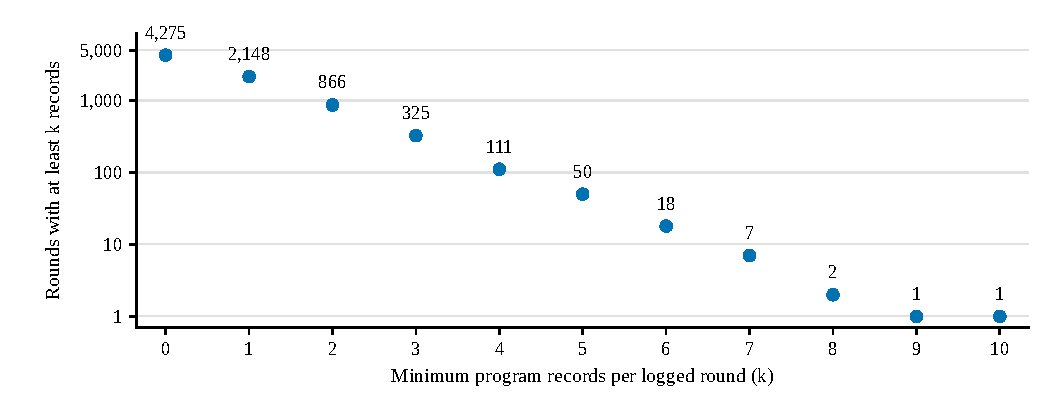
\includegraphics[width=\linewidth]{figures/fig_program_record_multiplicity.pdf}
  \caption{\textbf{Program-journal counts vary across the captured rounds.}
  All 3,529 ordinary program-promotion records across 4,275 logged round
  identifiers, 775--5049. Each point counts rounds with at least $k$ records,
  for every integer threshold from zero through the observed maximum, ten;
  the vertical count axis is logarithmic. At $k=0$, all 4,275 rounds enter;
  2,127 have no program record in this capture. The journals jointly cover
  every round identifier: 4,274 have scored adapter decisions, while round
  4331 has one program record and no recorded adapter decision. It remains
  included without inferring that decision. Counts are journal records,
  not distinct programs or proposal attempts; they establish neither
  independent tasks, success rates, elapsed time nor neural-writer or
  ranking-map learning. No points are fitted, smoothed or interpolated.
  Scope: the operating record through round 5049 in the main manuscript.}
  \label{fig:program-record-multiplicity}
\end{figure}
